% This file was converted to LaTeX by Writer2LaTeX ver. 1.0.2
% see http://writer2latex.sourceforge.net for more info
\documentclass[12pt]{article}
\usepackage[utf8]{inputenc}
\usepackage[T1]{fontenc}
\usepackage[english]{babel}
\usepackage{amsmath}
\usepackage{amssymb,amsfonts,textcomp}
\usepackage{array}
\usepackage{supertabular}
\usepackage{hhline}
\usepackage{hyperref}
\hypersetup{colorlinks=true, linkcolor=blue, citecolor=blue, filecolor=blue, urlcolor=blue}
\usepackage{graphicx}
% Text styles
\newcommand\textstylefamilyname[1]{#1}
\newcommand\textstyleStrong[1]{\textbf{#1}}
\newcommand\textstyleHTMLCite[1]{\textit{#1}}
\newcommand\textstyleappleconvertedspace[1]{#1}
\newcommand\textstyleslugpages[1]{#1}
\makeatletter
\newcommand\arraybslash{\let\\\@arraycr}
\makeatother
\raggedbottom
% Paragraph styles
\renewcommand\familydefault{\rmdefault}
\newenvironment{styleStandard}{\setlength\leftskip{0cm}\setlength\rightskip{0cm plus 1fil}\setlength\parindent{0cm}\setlength\parfillskip{0pt plus 1fil}\setlength\parskip{0in plus 1pt}\writerlistparindent\writerlistleftskip\leavevmode\normalfont\normalsize\writerlistlabel\ignorespaces}{\unskip\vspace{0.111in plus 0.0111in}\par}
\newenvironment{stylelsSectioni}{\setlength\leftskip{0.25in}\setlength\rightskip{0in plus 1fil}\setlength\parindent{0in}\setlength\parfillskip{0pt plus 1fil}\setlength\parskip{0.1665in plus 0.016649999in}\writerlistparindent\writerlistleftskip\leavevmode\normalfont\normalsize\fontsize{18pt}{21.6pt}\selectfont\bfseries\writerlistlabel\ignorespaces}{\unskip\vspace{0.0835in plus 0.00835in}\par}
\newenvironment{stylelsSourceline}{\renewcommand\baselinestretch{1.0}\setlength\leftskip{0.748in}\setlength\rightskip{0in plus 1fil}\setlength\parindent{0in}\setlength\parfillskip{0pt plus 1fil}\setlength\parskip{0in plus 1pt}\writerlistparindent\writerlistleftskip\leavevmode\normalfont\normalsize\itshape\writerlistlabel\ignorespaces}{\unskip\vspace{0in plus 1pt}\par}
\newenvironment{stylelsSectionii}{\setlength\leftskip{0.25in}\setlength\rightskip{0in plus 1fil}\setlength\parindent{0in}\setlength\parfillskip{0pt plus 1fil}\setlength\parskip{0.222in plus 0.0222in}\writerlistparindent\writerlistleftskip\leavevmode\normalfont\normalsize\fontsize{16pt}{19.2pt}\selectfont\bfseries\writerlistlabel\ignorespaces}{\unskip\vspace{0.0835in plus 0.00835in}\par}
\newenvironment{stylelsSectioniii}{\setlength\leftskip{0.5717in}\setlength\rightskip{0in plus 1fil}\setlength\parindent{0in}\setlength\parfillskip{0pt plus 1fil}\setlength\parskip{0.0972in plus 0.00972in}\writerlistparindent\writerlistleftskip\leavevmode\normalfont\normalsize\fontsize{14pt}{16.8pt}\selectfont\bfseries\writerlistlabel\ignorespaces}{\unskip\vspace{0in plus 1pt}\par}
\newenvironment{stylelsSectioniv}{\setlength\leftskip{0.25in}\setlength\rightskip{0in plus 1fil}\setlength\parindent{0in}\setlength\parfillskip{0pt plus 1fil}\setlength\parskip{0.0972in plus 0.00972in}\writerlistparindent\writerlistleftskip\leavevmode\normalfont\normalsize\bfseries\writerlistlabel\ignorespaces}{\unskip\vspace{0in plus 1pt}\par}
\newenvironment{stylelsEnumerated}{\renewcommand\baselinestretch{1.0}\setlength\leftskip{0cm}\setlength\rightskip{0cm plus 1fil}\setlength\parindent{0cm}\setlength\parfillskip{0pt plus 1fil}\setlength\parskip{0in plus 1pt}\writerlistparindent\writerlistleftskip\leavevmode\normalfont\normalsize\writerlistlabel\ignorespaces}{\unskip\vspace{0.0972in plus 0.00972in}\par}
\newenvironment{stylelsConversationTranscript}{\renewcommand\baselinestretch{1.0}\setlength\leftskip{0cm}\setlength\rightskip{0cm plus 1fil}\setlength\parindent{0cm}\setlength\parfillskip{0pt plus 1fil}\setlength\parskip{0in plus 1pt}\writerlistparindent\writerlistleftskip\leavevmode\normalfont\normalsize\writerlistlabel\ignorespaces}{\unskip\vspace{0.0972in plus 0.00972in}\par}
\newenvironment{stylelsTable}{\setlength\leftskip{0cm}\setlength\rightskip{0cm}\setlength\parindent{0cm}\setlength\parfillskip{0pt plus 1fil}\setlength\parskip{0.0201in plus 0.00201in}\writerlistparindent\writerlistleftskip\leavevmode\normalfont\normalsize\mdseries\writerlistlabel\ignorespaces}{\unskip\vspace{0in plus 1pt}\par}
% List styles
\newcommand\writerlistleftskip{}
\newcommand\writerlistparindent{}
\newcommand\writerlistlabel{}
\newcommand\writerlistremovelabel{\aftergroup\let\aftergroup\writerlistparindent\aftergroup\relax\aftergroup\let\aftergroup\writerlistlabel\aftergroup\relax}
\newcounter{listWWNumxxiileveli}
\newcounter{listWWNumxxiilevelii}[listWWNumxxiileveli]
\newcounter{listWWNumxxiileveliii}[listWWNumxxiilevelii]
\newcounter{listWWNumxxiileveliv}[listWWNumxxiileveliii]
\renewcommand\thelistWWNumxxiileveli{\arabic{listWWNumxxiileveli}}
\renewcommand\thelistWWNumxxiilevelii{\arabic{listWWNumxxiileveli}.\arabic{listWWNumxxiilevelii}}
\renewcommand\thelistWWNumxxiileveliii{\arabic{listWWNumxxiileveli}.\arabic{listWWNumxxiilevelii}.\arabic{listWWNumxxiileveliii}}
\renewcommand\thelistWWNumxxiileveliv{\arabic{listWWNumxxiileveli}.\arabic{listWWNumxxiilevelii}.\arabic{listWWNumxxiileveliii}.\arabic{listWWNumxxiileveliv}}
\newcommand\labellistWWNumxxiileveli{\thelistWWNumxxiileveli.}
\newcommand\labellistWWNumxxiilevelii{\thelistWWNumxxiilevelii.}
\newcommand\labellistWWNumxxiileveliii{\thelistWWNumxxiileveliii.}
\newcommand\labellistWWNumxxiileveliv{\thelistWWNumxxiileveliv.}
\newenvironment{listWWNumxxiileveli}{\def\writerlistleftskip{\addtolength\leftskip{0.0cm}}\def\writerlistparindent{}\def\writerlistlabel{}\def\item{\def\writerlistparindent{\setlength\parindent{-0cm}}\def\writerlistlabel{\stepcounter{listWWNumxxiileveli}\makebox[0cm][l]{\labellistWWNumxxiileveli}\hspace{0cm}\writerlistremovelabel}}}{}
\newenvironment{listWWNumxxiilevelii}{\def\writerlistleftskip{\addtolength\leftskip{0.0cm}}\def\writerlistparindent{}\def\writerlistlabel{}\def\item{\def\writerlistparindent{\setlength\parindent{-0cm}}\def\writerlistlabel{\stepcounter{listWWNumxxiilevelii}\makebox[0cm][l]{\labellistWWNumxxiilevelii}\hspace{0cm}\writerlistremovelabel}}}{}
\newenvironment{listWWNumxxiileveliii}{\def\writerlistleftskip{\addtolength\leftskip{0.0cm}}\def\writerlistparindent{}\def\writerlistlabel{}\def\item{\def\writerlistparindent{\setlength\parindent{-0cm}}\def\writerlistlabel{\stepcounter{listWWNumxxiileveliii}\makebox[0cm][r]{\labellistWWNumxxiileveliii}\hspace{0cm}\writerlistremovelabel}}}{}
\newenvironment{listWWNumxxiileveliv}{\def\writerlistleftskip{\addtolength\leftskip{0.0cm}}\def\writerlistparindent{}\def\writerlistlabel{}\def\item{\def\writerlistparindent{\setlength\parindent{-0cm}}\def\writerlistlabel{\stepcounter{listWWNumxxiileveliv}\makebox[0cm][l]{\labellistWWNumxxiileveliv}\hspace{0cm}\writerlistremovelabel}}}{}
\newcounter{listWWNumxleveli}
\newcounter{listWWNumxlevelii}[listWWNumxleveli]
\newcounter{listWWNumxleveliii}[listWWNumxlevelii]
\newcounter{listWWNumxleveliv}[listWWNumxleveliii]
\renewcommand\thelistWWNumxleveli{\arabic{listWWNumxleveli}}
\renewcommand\thelistWWNumxlevelii{\alph{listWWNumxlevelii}}
\renewcommand\thelistWWNumxleveliii{\roman{listWWNumxleveliii}}
\renewcommand\thelistWWNumxleveliv{\arabic{listWWNumxleveliv}}
\newcommand\labellistWWNumxleveli{\thelistWWNumxleveli.}
\newcommand\labellistWWNumxlevelii{\thelistWWNumxlevelii.}
\newcommand\labellistWWNumxleveliii{\thelistWWNumxleveliii.}
\newcommand\labellistWWNumxleveliv{\thelistWWNumxleveliv.}
\newenvironment{listWWNumxleveli}{\def\writerlistleftskip{\addtolength\leftskip{0.0cm}}\def\writerlistparindent{}\def\writerlistlabel{}\def\item{\def\writerlistparindent{\setlength\parindent{-0cm}}\def\writerlistlabel{\stepcounter{listWWNumxleveli}\makebox[0cm][l]{\labellistWWNumxleveli}\hspace{0cm}\writerlistremovelabel}}}{}
\newenvironment{listWWNumxlevelii}{\def\writerlistleftskip{\addtolength\leftskip{0.0cm}}\def\writerlistparindent{}\def\writerlistlabel{}\def\item{\def\writerlistparindent{\setlength\parindent{-0cm}}\def\writerlistlabel{\stepcounter{listWWNumxlevelii}\makebox[0cm][l]{\labellistWWNumxlevelii}\hspace{0cm}\writerlistremovelabel}}}{}
\newenvironment{listWWNumxleveliii}{\def\writerlistleftskip{\addtolength\leftskip{0.0cm}}\def\writerlistparindent{}\def\writerlistlabel{}\def\item{\def\writerlistparindent{\setlength\parindent{-0cm}}\def\writerlistlabel{\stepcounter{listWWNumxleveliii}\makebox[0cm][r]{\labellistWWNumxleveliii}\hspace{0cm}\writerlistremovelabel}}}{}
\newenvironment{listWWNumxleveliv}{\def\writerlistleftskip{\addtolength\leftskip{0.0cm}}\def\writerlistparindent{}\def\writerlistlabel{}\def\item{\def\writerlistparindent{\setlength\parindent{-0cm}}\def\writerlistlabel{\stepcounter{listWWNumxleveliv}\makebox[0cm][l]{\labellistWWNumxleveliv}\hspace{0cm}\writerlistremovelabel}}}{}
\setlength\tabcolsep{1mm}
\renewcommand\arraystretch{1.3}
% footnotes configuration
\makeatletter
\renewcommand\thefootnote{\arabic{footnote}}
\makeatother
\title{}
\author{Thomas-Wilhelm, Dakota J}
\date{2018-03-20}
\begin{document}
\title{\textsuperscript{Writing Performance \& time of Exposure in EFL Immersion Learners: Analysing Complexity, Accuracy, \& Fluency}}
\maketitle

\begin{styleStandard}
\textit{Isabel Tejada-S}\textit{ánchez}\textit{\textsuperscript{1}}\textit{ \& Carmen Pérez-Vidal}\textit{\textsuperscript{2}}
\end{styleStandard}

\begin{styleStandard}
\textsuperscript{1}Universidad de los Andes, \textsuperscript{2}Universitat Pompeu Fabra
\end{styleStandard}

\begin{stylelsSectioni}
Abstract
\end{stylelsSectioni}


\begin{stylelsSourceline}
The present study explores the effects of two types of early-partial immersion programmes on writing performance in English as a Foreign Language (EFL). It examines adolescent learners (ages 12-17) in mainstream education in Colombia. The two programmes are similar as far as the learners’ onset age (4) is concerned, but different with respect to the total amount of EFL exposure time and intensity: High Intensity plus (HI+) has a total of 8,760 accumulated hours by age 17, while High Intensity (HI) has in turn, 7,002. It has been prevalently hypothesized that the more time students dedicate to learning the L2, the higher their level of proficiency will be (Carroll 1962, Stern 1985), supporting the spread of instructed immersion and intensive programmes (Serrano, Llanes \& Tragant 2011, Lightbown 2012); one of the aims of this chapter is to further assess this hypothesis. \ The study examines a cross-sectional sample (N=188), adopting a between-groups design whereby programmes’ performance is compared in terms of the effect of accumulated time. Analysis will focus on the domains of syntactic and lexical complexity, accuracy, fluency (Housen, Kuiken \& Vedder 2012) and on holistic ratings. Results indicate that learners’ writing in HI+ and HI do not show to be significantly different in most domains of CAF examined, nor in the holistic ratings. This might be explained in the light of the prior high number of accumulated hours of English exposure and emphasis on literacy in the curriculum of both programmes, which has allowed learners to reach a threshold level from which they do not regress (Bournot-Trites 2007, Williams 2012).
\end{stylelsSourceline}

\setcounter{listWWNumxxiileveli}{0}
\begin{listWWNumxxiileveli}
\item 
\begin{stylelsSectioni}
Introduction
\end{stylelsSectioni}

\end{listWWNumxxiileveli}
\begin{styleStandard}
Since the emergence of immersion programmes in Canada in the late 1960s (Lambert \& Tucker 1972), much research has been carried out on the development of linguistic competence in an L2 in such settings (Genesee 1976; 1978, Swain 2000). The majority of these studies, mostly in favour of immersion, have also addressed the limitations of immersion programmes, particularly in terms of the L2 competence attained and the risks involved in the development of the L1 (Genesee 1978; 2013, Lazaruk 2007). Despite these concerns, the immersion education model has developed rapidly, inspiring bi- and multilingual school programmes throughout the world (De Mejia 2002). The acknowledged success of immersion programmes may be due to a combination of factors that have been shown to positively affect L2 acquisition, such as onset age, the type of input made available and its quantity, that is, the amount of time allocated to L2 exposure, methodological flexibility (early, middle and late programmes) and teachers’ backgrounds, among others (Genesee 2013, Johnson \& Swain 1997, Lazaruk 2007). 
\end{styleStandard}

\begin{styleStandard}
This chapter is part of a larger study (Tejada-Sánchez 2014) which examines \ the outcomes of immersion programmes in Colombia, focusing on EFL writing of L1-Spanish speakers. More specifically, it seeks to understand the relationship between the allocation of time in the programme and the resulting learners’ written performance in their target language, English. This relationship has not been sufficiently addressed in studies on school immersion contexts outside Canada, and even less so in the Colombian context. Earlier studies and compilations have underscored the importance of addressing the effect of the time factor, and more specifically intensive exposure experiences, within L2 instructional settings (Muñoz 2012). \ Consequently, there remains a gap in the literature as to how language productive abilities benefit from such intensive instructional experiences. Undoubtedly, the number of uncontrollable variables within educational settings, such as individual differences, curriculum and context specifics, make this a particularly complex endeavour. For this study, data collection was conducted during class time in order to ensure the students’ participation. It included written data and a background questionnaire which was used to control for individual variables such as age, L2 exposure and target language contact hours outside the school. \ \ \ \ 
\end{styleStandard}

\begin{styleStandard}
The chapter thus presents a descriptive study that evaluates the relative effect of different amounts of exposure to L2-English in two early partial immersion programmes in Colombia. We begin by reviewing the literature concerning time as an essential factor within immersion programmes, to then go on to discuss writing development in terms of the CAF triad, as well as the measurements adopted for profiling these dimensions. We then move on to present the methodology. Finally, results and analysis are outlined, followed by a discussion. Concluding remarks will focus on the implications of this study for L2 education and specifically curriculum allocation of languages within immersion programmes in non-English speaking contexts.
\end{styleStandard}

\begin{listWWNumxxiileveli}
\item 
\begin{stylelsSectioni}
Literature review
\end{stylelsSectioni}


\setcounter{listWWNumxxiilevelii}{0}
\begin{listWWNumxxiilevelii}
\item 
\begin{stylelsSectionii}
Time as an intrinsic factor for immersion programmes
\end{stylelsSectionii}

\end{listWWNumxxiilevelii}
\end{listWWNumxxiileveli}
\begin{styleStandard}
The question of the influence of the amount of target language exposure on language proficiency was raised quite early in the implementation of French immersion programmes in Canada. Carroll’s contributions in the mid-sixties and seventies around the characteristics of immersion programmes were fundamental. Regarding the time-skill relationship, he asserted: “There are many factors which contribute directly to the effectiveness of French instructional programs (...) Organizationally, it is considered \textit{that the key factor is the number of hours of instruction} in French (…) In other words, \textit{the more hours a pupil spends in French, the higher level of achievement is likely to b}\textit{e}” (Carroll 1977: 8, cited in Swain 1981: 2-3; emphasis added). He identified a direct link between the volume of input made available to learners, quantified as time, and the overall L2 attainment. Stern (1985), in turn, referred to a threshold regarding the number of hours likely to ensure a \textit{bilingual} competence in an immersion context: at least 5,000 hours, but this account did not determine the characteristics of the learner involved in the programme, and did not make explicit the distribution of exposure time or its intensity, in terms of hours per week/month. Currently, the publications which explore time as a factor in the development of an L2 emphasize its importance but at the same time its intricate complexity. \ The conclusions that can be drawn from Muñoz’s (2012) compilation demonstrate that, depending on how and where time is operationalized in language education, it can lead to a myriad of effects, from cognitive to socio-pragmatic, from global language features to discrete ones such as those addressed by the CAF dimensions. In this study, we focus on the parameter of accumulated time of exposure\textit{.} This parameter refers to the global amount of time, in terms of number of hours, dedicated to L2 learning (Stern 1985, Genesee 1974; 1978; 2013). It is usually required for the completion of a programme with a given target proficiency level, as defined for instance by the CEFR descriptors (Council of Europe 2001). \ Regarding the accumulated time of exposure, immersion programmes are those where L2-contact time, along with content integrated instruction, is deemed essential for the programme’s functioning (Collins, Halter, Lightbown \& Spada 1999). Globally, immersion programmes have been traditionally described as beneficial for receptive skills (Day \& Shapson 1988), while their limitations regarding writing and accuracy have been frequently reported in previous research (Lightbown 2012; Germain, Netten \& Séguin 2004). In such respect, in written and oral expression, immersion learners often demonstrate a considerable influence of L1 grammar. Also, it has been repeatedly reported that learners would not start a conversation in the L2 spontaneously, unless when they are asked to do so (Harley 1992, Wesche 2002). Finally, it is suggested that even though productive skills appear to be distant from those of native speakers, learners in immersion programmes continue to make progress in the L2 (Harley 1992, Wesche 1989, Housen 2012).
\end{styleStandard}

\begin{styleStandard}
Particularly in terms of writing, the main topic in this study, contributions by Bournot-Trites (2007), Collins \& White (2011), Turnbull, Lapkin, Hart \& Swain (1998) and Lightbown (2012) underscore learners’ capability to communicate effectively but failing to reach native-like levels, for instance as regards lexical diversity and structural elaboration. \ 
\end{styleStandard}

\begin{styleStandard}
Summing up, it has been prevalently hypothesized that the more time students dedicate to learning the L2, the higher their level of proficiency will be (Stern 1985), thus supporting the spread of instructed immersion and intensive programmes (Serrano et al. 2011, Lightbown 2012). However, although the pioneer Canadian initiatives have been abundantly documented in the SLA literature, research is scarce as far as other countries are concerned. Hence, the current study seeks to shed light on the effects of EFL immersion in Colombia, by examining and comparing the effects on writing performance of students belonging to two programmes which differ in total number of hours and their distribution. Individual differences such as L2 exposure outside school, family bilingualism, and total amount of time in the school were also taken into consideration, but will not be discussed in this chapter.
\end{styleStandard}

\begin{listWWNumxxiileveli}
\item 
\setcounter{listWWNumxxiilevelii}{0}
\begin{listWWNumxxiilevelii}
\item 
\begin{stylelsSectionii}
L2 Written performance
\end{stylelsSectionii}

\end{listWWNumxxiilevelii}
\end{listWWNumxxiileveli}
\begin{styleStandard}
Writing is a cognitively complex and multidimensional endeavour which involves different stages and processes (Manchón 2013, Ortega 2012). In fact, this skill is understood as an {\textquotesingle}interactive{\textquotesingle} process where various factors, such as genre awareness (stylistic organization and textual format) and mastery of content and language, are frequently activated and deactivated, according to writing pace and the needs of the composition process.
\end{styleStandard}

\begin{styleStandard}
Creating a text comprises three main stages, namely, planning, formulation and revision (Manchón 2009; 2013, Silva \& Matsuda 2005). In the case of an L2, this activity is complicated by additional demands such as the search for the appropriate lexicon, grammar, discourse and other peculiar dimensions of the target language and culture (Manchón 2009). 
\end{styleStandard}

\begin{styleStandard}
In this study, writing is seen as a genuine and meaningful way of communication in controlled L2 settings, such as the immersion school. Thus, in line with Harklau (2002), Ortega (2012) and Williams (2012), writing is a means of promoting permanent opportunities for practicing and revising L2 production in the classroom. 
\end{styleStandard}

\begin{styleStandard}
Two main approaches have been used to analyse writing in this study: quantitative measures for the three CAF dimensions and qualitative assessment using holistic ratings.
\end{styleStandard}

\begin{listWWNumxxiileveli}
\item 
\setcounter{listWWNumxxiilevelii}{0}
\begin{listWWNumxxiilevelii}
\item 
\begin{stylelsSectionii}
Complexity, accuracy, and fluency (CAF)
\end{stylelsSectionii}

\end{listWWNumxxiilevelii}
\end{listWWNumxxiileveli}
\begin{styleStandard}
The quest for a developmental index to describe L2 performance has been a key issue in SLA research for decades now (among the first attempts, see e.g. Larsen-Freeman 1978). Building on \ models of L2 proficiency (Skehan 2009, Ellis \& Barkhuizen 2005, among others), Housen et al’s 2012 volume elaborates on the potential of CAF as complementary dimensions of language performance and as a reliable approach to gauging L2 proficiency, as the three dimensions encompass the major areas of performance in an interlanguage system. 
\end{styleStandard}

\begin{styleStandard}
In this study, we adopt the CAF triad to assess writing performance in immersion contexts. Several contributions (Bulté \& Housen 2014, Housen \& Kuiken 2009, Housen et al. 2012, Wolfe-Quintero, Inagaki \& Kim 1998), have discussed the operationalization of these measures in order to explain what makes a learner a \textit{skilled} user of a language. Below we review those adopted for our study. \ 
\end{styleStandard}

\begin{listWWNumxxiileveli}
\item 
\begin{stylelsSectioniii}
Complexity
\end{stylelsSectioniii}

\end{listWWNumxxiileveli}
\begin{styleStandard}
Complexity is a construct that reflects the multidimensionality of the language learning process. It particularly poses numerous problems in the SLA field due to its polysemic nature, which can refer to structural, cognitive and developmental aspects (Pallotti 2015).
\end{styleStandard}

\begin{styleStandard}
In this study, L2 complexity is analysed from the language structure point of view claimed by Housen et al. (2012) and Pallotti (2015). This implies looking at the properties of L2 constructions, forms, \ form-meaning mappings and their interrelationships. \ 
\end{styleStandard}

\begin{styleStandard}
Several accounts have discussed the multiple operationalisations of this construct and underscored its problematic nature (i.e. Wolfe-Quintero et al. 1998, Norris \& Ortega 2009, Pallotti 2015, Housen et al. 2012, Skehan 2009). In this respect, a wealth of measurements have been applied, revealing relatively operationalization vagueness and ‘low content validity’ (Bulté \& Housen 2014: 47). Its multicompositional nature implies that complexity operates based on major assumptions that include: ‘the more content means more complex’, or ‘the longer’, ‘the most embedded’ or the ‘more varied’, all imply more complexity. As Bulté \& Housen (2014) emphasize when examining short-term changes in written complexity, L2 research needs to be cautious about the validity of such measures and their implications, as their predictions may vary depending on the context, the learner and the task. 
\end{styleStandard}

\begin{styleStandard}
In light of these observations, this study seeks to adopt complexity as an indicator of L2 performance at different stages of language instruction. The selection of measures for syntactic and lexical complexity takes into account the nature of \ the texts produced by different groups of learners, which, in our study are often rather short.
\end{styleStandard}

\begin{listWWNumxxiileveli}
\item 
\setcounter{listWWNumxxiilevelii}{0}
\begin{listWWNumxxiilevelii}
\item 
\setcounter{listWWNumxxiileveliii}{0}
\begin{listWWNumxxiileveliii}
\item 
\setcounter{listWWNumxxiileveliv}{0}
\begin{listWWNumxxiileveliv}
\item 
\begin{stylelsSectioniv}
Syntactic complexity
\end{stylelsSectioniv}

\end{listWWNumxxiileveliv}
\end{listWWNumxxiileveliii}
\end{listWWNumxxiilevelii}
\end{listWWNumxxiileveli}
\begin{styleStandard}
Syntactic complexity is generally measured through the length, proportion, combination and interrelation of \ different elements within a text (Bulté \& Housen 2014). Several elements or units have been taken into consideration such as the sentence, the clause and the T-Unit, among others. \ Following Pallotti (2015), this study examines L2 syntactic complexity by analysing structural properties at the sentential and the clausal level as well as text organisation properties through the use of coordination and subordination. Therefore, following Torras, Navés, Celaya \& Pérez-Vidal (2006) the measurements adopted for the study were independent and dependent clauses per sentence (IndepCS and DepCS), and, following Bulté \& Housen (2014), the Coordinated Clause Ratio (CoordCR) calculated by dividing the number of coordinated clauses by the number of sentences. As argued by Bulté \& Housen (2012; 2014) this type of calculation (CoordCR) highlights the use of coordination within a text and differs from the Coordination Index developed by Bardovi-Harlig (1992) in that the CI appears to be a measure of clause combination that entails subordination as well: “the score on this index depends on the amount of subordination produced” (Bulté \& Housen et al. 2012 p. 38).
\end{styleStandard}

\begin{listWWNumxxiileveli}
\item 
\setcounter{listWWNumxxiilevelii}{0}
\begin{listWWNumxxiilevelii}
\item 
\setcounter{listWWNumxxiileveliii}{0}
\begin{listWWNumxxiileveliii}
\item 
\setcounter{listWWNumxxiileveliv}{0}
\begin{listWWNumxxiileveliv}
\item 
\begin{stylelsSectioniv}
Lexical complexity
\end{stylelsSectioniv}

\end{listWWNumxxiileveliv}
\end{listWWNumxxiileveliii}
\end{listWWNumxxiilevelii}
\end{listWWNumxxiileveli}
\begin{styleStandard}
Lexical complexity has been frequently analysed by looking at lexical diversity, density and sophistication (Housen et al. 2012, Bulté \& Housen 2014). Diversity,\textit{ }also known as lexical range (Crystal 1982) or lexical variation (Read 2000), is measured through calculations which account for the variety of vocabulary items within a language sample (Malvern, Richards, Chipere \& Duran 2004). Measurements of density and sophistication are mostly used either with larger text samples or to discriminate amongst text genres (Read 2000). Nonetheless, it has also been argued that these measures do not really operationalize structural complexity. As Pallotti (2015: 126) highlights, “indices of lexical sophistication, like the percentage of rare or difficult words, may be valid indicators of development, but they do not directly tap structural complexity; from a structural point of view, a rare word like \textit{tar} is not in itself more complex than a common one like \textit{car}.” Today, there is a general consensus in that diversity, sophistication and density (and an additional dimension of lexical accuracy) allow us to profile vocabulary development. In addition, diversity has been frequently examined with shorter texts such as those in our data (Meara and Miralpeix 2017).This is then the measure we have adopted to assess lexical complexity in this study.
\end{styleStandard}

\begin{styleStandard}
Thus, this study uses two measures of diversity to gauge learners’ lexical repertoire. First, \textit{Guiraud’s Index,} which results from dividing the number of types by the square root of the tokens in order to limit text size effects. The second one is D, computed with the \textit{vocd} tool in CLAN (MacWhinney 2000), which estimates lexical distribution in longer text samples (Malvern \& Richards 2000). \ Both measures have been used used to gauge language diversity in general; however, consensus has not been reached over which index proves to be a better predictor of lexical diversity in a person’s interlanguage (McCarthy \& Jarvis 2010, in Pallotti 2015). Therefore, this study will report both measures, to provide a more comprehensive picture.
\end{styleStandard}

\begin{listWWNumxxiileveli}
\item 
\begin{stylelsSectioniii}
Accuracy
\end{stylelsSectioniii}

\end{listWWNumxxiileveli}
\begin{styleStandard}
The accuracy domain refers to the appropriateness of grammatical, lexical, semantic and pragmatic choices with respect to L2 target parameters. It is one of the most observed traits in the language production of L2 learners and it has been frequently treated as a key aspect of interlanguage development (Housen et al. 2012). Accuracy is operationalised by counting the grammatical and lexical errors in a linguistic production. However, Polio (1997; 2001) remarks that the most commonly used measure for this domain is the quantity of units with no errors (Error-Free units), which poses problems for the analysis of short compositions or those by beginner learners. In this study, overall measures of specific errors such as total amount of errors per 100 words and Grammar errors per 100 words (ToralErr/100 and GrErr/100) were calculated, \ as they capture the totality of errors produced as well as their structural category. Grammatical errors were predominant in most of the scripts, and they mainly corresponded to agreement phenomena and verb conjugations.
\end{styleStandard}

\begin{listWWNumxxiileveli}
\item 
\begin{stylelsSectioniii}
Fluency
\end{stylelsSectioniii}

\end{listWWNumxxiileveli}
\begin{styleStandard}
This term is commonly associated with the speed of articulation, rhythm, and pausing in the production of oral language. In the case of written compositions, it refers to the \ length of units, that is, the quantity of words and structures produced within a given time (Bulté \& Housen 2014). To account for written fluency, this study adopts the view whereby the proportion of words produced is observed in relation to a given amount of time (task time, which in our case was 20 minutes). Previous research employed measures such as the number of units produced per minute, or the number of units produced within a ‘macro’ structure such as the sentence; in the present study, \ measurements in this domain include words per minute and words per sentence (WM and WS). These measures provide an account of fluency in terms of quantity and rate of production. These were chosen over analogous proposals such as \textit{words per burst, }defined as the number of written words produced between two pauses or other interruptions (Gunnarson 2012), as the scripts analysed for this study were not collected using key-logging technologies.
\end{styleStandard}

\begin{listWWNumxxiileveli}
\item 
\setcounter{listWWNumxxiilevelii}{0}
\begin{listWWNumxxiilevelii}
\item 
\begin{stylelsSectionii}
Holistic ratings
\end{stylelsSectionii}

\end{listWWNumxxiilevelii}
\end{listWWNumxxiileveli}
\begin{styleStandard}
Holistic \ approaches to the evaluation of L2 writing have frequently been used in SLA research. These can be operationalised through scoring carried out by trained raters following assessment rubrics. These instruments usually consist of descriptors of the language used by the learner as well as the degree of completion of a given task. For example, standardized tests’ examination grids, (e.g. TOEFL) include various indicators that reflect a learner{\textquotesingle}s L2 competence according to specific criteria, purpose and genre. In L2 research, these ratings often serve as complements to objective measurements of text quality (Weigle 2002). \ 
\end{styleStandard}

\begin{styleStandard}
Our study uses a scoring rubric for the qualitative assessment of learners’ written composition (Friedl \& Auer 2007). This scale examines the characteristics of beginner to high intermediate levels of expository and narrative composition, also including task completion criteria. It was originally designed for the evaluation of English-L2 written performance within CLIL school settings in Austria (Friedl \& Auer 2007, Dalton-Puffer, Nikula \& Smit 2010) and later on in Catalunya (Juan-Garau \& Salazar-Noguera 2015, Roquet \& Pérez-Vidal 2015). Four aspects are evaluated on a global scale of 0 to 20, which is in turn divided into four subscales ranging from 0 to 5: 1. Task fulfilment, 2. Text Organisation, 3. Grammar and 4. Vocabulary. \ In the current study this instrument has been adopted to profile learners’ descriptive writing within content-based instruction contexts, which are highly comparable to the contexts for which it was originally developed (Pérez-Vidal 2015).
\end{styleStandard}

\begin{listWWNumxxiileveli}
\item 
\begin{stylelsSectioni}
Research question
\end{stylelsSectioni}

\end{listWWNumxxiileveli}
\begin{styleStandard}
This study explores the relationship between L2 exposure time and writing performance in immersion learners, as measured through the CAF constructs and holistic ratings. Hence, the guiding research question is: \ 
\end{styleStandard}

\setcounter{listWWNumxleveli}{0}
\begin{listWWNumxleveli}
\item 
\begin{stylelsEnumerated}
Does accumulated time of EFL exposure in two contrasting immersion programmes (HI and HI+) have a differential impact in the long run on the learners’ writing performance, when assessed with a) CAF measures and b) holistic ratings? 
\end{stylelsEnumerated}

\end{listWWNumxleveli}
\begin{styleStandard}
On the basis of this question and our review of the literature we hypothesize that, at any given time that learners are measured in the respective programmes, the higher the number of accumulated hours of EFL exposure students receive, the higher their level of proficiency will be.
\end{styleStandard}

\setcounter{listWWNumxxiileveli}{0}
\begin{listWWNumxxiileveli}
\item 
\begin{stylelsSectioni}
Method
\end{stylelsSectioni}


\setcounter{listWWNumxxiilevelii}{0}
\begin{listWWNumxxiilevelii}
\item 
\begin{stylelsSectionii}
Context and participants
\end{stylelsSectionii}

\end{listWWNumxxiilevelii}
\end{listWWNumxxiileveli}
\begin{styleStandard}
Foreign language education is a central theme in Colombia’s political agenda (Bonilla \& Tejada 2016). English plays a major role in a long-term education project entitled \textit{Colombia Bilingüe}, which aims to rank Colombia as the highest provider of quality in education in Latin America. \ \ 
\end{styleStandard}

\begin{styleStandard}
Our study focussed on two immersion programmes with different total times of EFL exposure. We have named them High Intensity (N=52) and High Intensity \textit{plus} (N=136) (HI and HI+) for the purpose of the study\footnote{ The designation of these programmes has been adopted from Collins et al. (1999), Bournot-Trites (2007), and Collins and White (2011). \par }. The difference in the number of participants in both programmes is due to a larger pool of students in the schools following the HI+ programme. Table 1 displays the number of participants per programme, age-group, and grade involved. Both programmes represent actual implementations of immersion models in the private sector of Colombia’s educational system, with rather high amounts of L2 exposure compared to the average Colombian traditional EFL programmes. In the public sector, time of L2 instruction ranges in average from 2 to 4 hours per week, whereas in the private sector these amounts of L2-exposure are much higher, ranging from 7 to 20 hours per week, with L2 content-based instruction being predominant. 
\end{styleStandard}

\begin{center}
\tablehead{}
\begin{supertabular}{m{1.2011598in}m{0.6101598in}m{0.41365984in}m{0.70805985in}}
\centering \bfseries Age-group &
\centering \bfseries Grade &
\centering {\bfseries N}\par

\centering \bfseries HI+ &
\centering {\bfseries N}\par

\centering\arraybslash \bfseries HI\\\hline
\centering \bfseries 12 &
\centering 6\textsuperscript{th} &
\centering 12 &
\centering\arraybslash 14\\
\centering \bfseries 14 &
\centering 7\textsuperscript{th} &
\centering 34 &
\centering\arraybslash 8\\
\centering \bfseries 15 &
\centering 8\textsuperscript{th} &
\centering 22 &
\centering\arraybslash 8\\
\centering \bfseries 16 &
\centering 9\textsuperscript{th} &
\centering 20 &
\centering\arraybslash 5\\
\centering \bfseries 17 &
\centering 10\textsuperscript{th} &
\centering 48 &
\centering\arraybslash 17\\
\centering \bfseries Total &
\centering 11\textsuperscript{th} &
\centering 136 &
\centering\arraybslash 52\\
\end{supertabular}
\end{center}
\begin{styleStandard}
\textit{Table 1: }\textit{Number of participants per programme.}
\end{styleStandard}

\begin{styleStandard}
HI and HI+ follow an early partial EFL immersion model in an otherwise Spanish curriculum, the official language in Colombia. \ Schooling begins at the age of four in kindergarten. From this age onwards, courses are taught about 50\% of the time in the L2 and the other 50\% in the L1. The most significant exposure to the L2 is offered mainly through immersion instruction, that is through curricular content taught in English. In neither programme is English taught through a grammatical or metalinguistic approach. \ Interestingly, students seldom use the L2 outside the classroom or for non-academic activities, so there is little or none informal learning. 
\end{styleStandard}

\begin{styleStandard}
Figure 1 displays the mean L2-instruction hours per year\textit{ }in both programmes. Black refers to HI+ and light grey refers to HI. Primary school, which lasts five years (1\textsuperscript{st} to 5\textsuperscript{th }grade), is the most intense period in terms of L2 exposure, as most of the subject areas (Sciences, History, Arts, etc.) are taught in English in both programmes. In terms of time distribution in primary school, HI+ provides between 600 and 670 hours of L2-exposure per year, whereas HI provides 504 hours. High-school (6\textsuperscript{th} to 11\textsuperscript{th} grade) is characterized by a decrease in L2-instruction time in both programmes. The HI+ programme offers 372 hours of L2-instruction per year by the end of this stage, while the HI offers 288 hours. 
\end{styleStandard}

\begin{center}
 [Warning: Image ignored] % Unhandled or unsupported graphics:
%\includegraphics[width=4.7291in,height=2.9492in,width=\textwidth]{tejada-img1.wmf}

\end{center}
\begin{styleStandard}
\textit{Figure 1: }\textit{Mean L2-instruction hours per school year for programmes HI and HI+.}\textit{ }\ 
\end{styleStandard}

\begin{styleStandard}
Regarding the curriculum at higher stages, both the HI+ and HI programmes coincide in that the only subject areas taught in English during high school are \textit{English Language Arts} or \textit{Anglo-Saxon Literature}. These are offered in the L2 from 9\textsuperscript{th} grade on in both programmes (around age 15). Opportunities for exposure to English at other locations in the schools, for example in the school cafeteria, the playground or common areas remains limited. 
\end{styleStandard}

\begin{styleStandard}
\textit{The HI+ programme} gathers students from three schools. These offer the largest number of hours of L2 exposure-instruction time: \textbf{8760 accumulated hours }by the end of grade 11 (age 17). At the end of a school in the HI+ programme, a renowned international certification is provided\footnote{ The \textit{International Baccalaureate} certification (IB). In order to reach such a goal, these students from HI+ must follow the program for another year, grade 12, which was not considered in this study.}. 
\end{styleStandard}

\begin{styleStandard}
\textit{The HI programme }involves students from one school. It offers a relatively lower number of hours of L2 exposure-instruction time, \textbf{7002} \textbf{accumulated hours} by the end of grade 11 (age 17). A singular academic approach to literacy in the HI curriculum is underscored by the school’s stakeholders (principals, coordinators and teachers), so students are frequently exposed to discourse and text analysis since primary school. Table 2 shows the distribution of hours per year and the accumulated hours in the two programmes. 
\end{styleStandard}

\begin{flushleft}
\tablehead{}
\begin{supertabular}{m{0.6101598in}m{0.41435984in}m{0.41365984in}m{0.41435984in}m{0.41365984in}m{0.41435984in}m{0.7059598in}}
 &
\multicolumn{6}{m{3.1700597in}}{\bfseries Mean accumulated L2 hours per programme}\\
\bfseries Grade &
\mdseries 6th &
\mdseries 7th &
\mdseries 8th &
\mdseries 9th &
\mdseries 10th &
{\mdseries 11th}

\\
\bfseries Age  &
{\mdseries 12}

 &
\mdseries 13 &
\mdseries 14 &
\mdseries 15 &
\mdseries 16 &
\mdseries 17\\
\bfseries HI &
\mdseries 4914 &
\mdseries 5418 &
\mdseries 5922 &
\mdseries 6426 &
\mdseries 6714 &
{\mdseries 7002}

\\
\bfseries HI+ &
\mdseries 6312 &
\mdseries 6924 &
{\mdseries 7536}

 &
{\mdseries 8016}

 &
\mdseries 8388 &
\mdseries 8760\\
\end{supertabular}
\end{flushleft}
\begin{styleStandard}
\textit{Table 2. }\textit{Number}\textit{ of hours of L2 accumulated per year per programme.}
\end{styleStandard}

\begin{listWWNumxxiileveli}
\item 
\setcounter{listWWNumxxiilevelii}{0}
\begin{listWWNumxxiilevelii}
\item 
\begin{stylelsSectionii}
Design and procedure
\end{stylelsSectionii}

\end{listWWNumxxiilevelii}
\end{listWWNumxxiileveli}
\begin{styleStandard}
Written data was collected from five different age-groups (ages 12, 14, 15, 16, and 17) in each programme. Age 13 was not taken into consideration since the data collection process could not be completed with the whole group in one of the programmes.
\end{styleStandard}

\begin{listWWNumxxiileveli}
\item 
\begin{stylelsSectioniii}
Data collection and trimming
\end{stylelsSectioniii}

\end{listWWNumxxiileveli}
\begin{styleStandard}
Two main instruments were used to collect the data used for the present study: a linguistic background questionnaire and a written task consisting of a composition based on a silent film.
\end{styleStandard}

\begin{listWWNumxxiileveli}
\item 
\setcounter{listWWNumxxiilevelii}{0}
\begin{listWWNumxxiilevelii}
\item 
\setcounter{listWWNumxxiileveliii}{0}
\begin{listWWNumxxiileveliii}
\item 
\setcounter{listWWNumxxiileveliv}{0}
\begin{listWWNumxxiileveliv}
\item 
\begin{stylelsSectioniv}
Linguistic background questionnaire
\end{stylelsSectioniv}

\end{listWWNumxxiileveliv}
\end{listWWNumxxiileveliii}
\end{listWWNumxxiilevelii}
\end{listWWNumxxiileveli}
\begin{styleStandard}
A general linguistic background questionnaire inspired by Grosjean (2010) was used to investigate participants’ use of different languages, their learning habits, their L2 interaction and contact with target language speakers, as well as the average time spent in the immersion programme. This instrument was later used to make a selection of participants in the study. Students who had not been in the same school for their complete tuition (from primary years onwards), had lived in an English-speaking country or abroad, were binational or had English-speaking relatives, were excluded from the study. This left a final sample of 188 students including both programmes, as shown in Table 1.
\end{styleStandard}

\begin{listWWNumxxiileveli}
\item 
\setcounter{listWWNumxxiilevelii}{0}
\begin{listWWNumxxiilevelii}
\item 
\setcounter{listWWNumxxiileveliii}{0}
\begin{listWWNumxxiileveliii}
\item 
\setcounter{listWWNumxxiileveliv}{0}
\begin{listWWNumxxiileveliv}
\item 
\begin{stylelsSectioniv}
The writing task: Retelling a story
\end{stylelsSectioniv}

\end{listWWNumxxiileveliv}
\end{listWWNumxxiileveliii}
\end{listWWNumxxiilevelii}
\end{listWWNumxxiileveli}
\begin{styleStandard}
In order to collect data on the participants’ written abilities, they were asked to write a story retell on the basis of the silent film {\textquotedbl}College{\textquotedbl} (Horne \& Keaton 1927), starring Buster Keaton. The choice for this task emerged from earlier analyses on task structure such as Skehan \& Foster (1999), where narrative retellings tasks supported by visual prompts are used to elicit the three dimensions of CAF in comparable degrees. Likewise, silent films have frequently been used in SLA studies to elicit narratives in the L2 (e.g. \textstylefamilyname{Lambert}\textstyleStrong{\textmd{ }}\textstylefamilyname{1997, who used Chaplin’s Modern Times)}. 
\end{styleStandard}

\begin{styleStandard}
Participants watched a 3.30-minute scene of the film, which was played only once. Subsequently, they were allowed 20 minutes to complete the composition. They were asked to write as much as they were able to in the given time. They received the following instruction: 
\end{styleStandard}

\setcounter{listWWNumxleveli}{0}
\begin{listWWNumxleveli}
\item 
\begin{stylelsEnumerated}
Retell the story in writing while keeping in mind all the details. Use your current knowledge of English; do not use the dictionary. \ 
\end{stylelsEnumerated}

\end{listWWNumxleveli}
\setcounter{listWWNumxxiileveli}{0}
\begin{listWWNumxxiileveli}
\item 
\begin{stylelsSectioniii}
Data coding and analysis
\end{stylelsSectioniii}

\end{listWWNumxxiileveli}
\begin{styleStandard}
All the participants’ compositions (N=188) collected through the written tasks were transcribed and coded using CLAN (MacWhinney 2000). A first streamlining was conducted to standardize coding procedures. L2 errors and spelling occurrences were identified and scripts were segmented into units. The errors that were not taken into account were those caused by phonology or graphical ambiguity (i.e. \textit{the man say{\textquotesingle}s}), misspelling (i.e. \textit{he whent}), redundancy, or repetition of text content (i.e. \textbf{\textit{A man}}\textit{ put a poster that says Boy needed. And then }\textbf{\textit{a man}}\textit{ come and tell that he want the work}). 
\end{styleStandard}

\begin{styleStandard}
CAF measures and holistic ratings were employed to analyse the learners’ writings. CAF analysis was carried out through manual coding of grammatical and lexical errors, segmentation of syntactic units and automatic calculations using CLAN and Excel. Holistic ratings were carried out by two external evaluators. In order to compare learners’ performance in terms of the impact of the accumulated time of exposure in HI and HI+, \ descriptive statistics (means and SDs) were calculated on both CAF measures and holistic ratings for all the age groups combined (12, 14, 15, 16, and 17) in each programme, which allowed us to measure the effects throughout the programme. Between-groups comparisons were conducted using Welch’s t-test.
\end{styleStandard}

\begin{listWWNumxxiileveli}
\item 
\setcounter{listWWNumxxiilevelii}{0}
\begin{listWWNumxxiilevelii}
\item 
\setcounter{listWWNumxxiileveliii}{0}
\begin{listWWNumxxiileveliii}
\item 
\setcounter{listWWNumxxiileveliv}{0}
\begin{listWWNumxxiileveliv}
\item 
\begin{stylelsSectioniv}
The unit of analysis
\end{stylelsSectioniv}

\end{listWWNumxxiileveliv}
\end{listWWNumxxiileveliii}
\end{listWWNumxxiilevelii}
\end{listWWNumxxiileveli}
\begin{styleStandard}
The main unit of analysis in our study is the sentence. Our scripts resulted in an average of 32 words (see Table 3), which made an analysis based on T-Units (Hunt 1965) too restraining, as this syntactic unit requires longer compositions to allow for a more substantive examination of how the units are conceived by the writer in terms of length and interrelations between clauses. Following Bardovi-Harlig (1992), this study adopts the sentence as the main syntactic unit in order to keep the author’s original textual/syntactic segmentation. 
\end{styleStandard}

\begin{styleStandard}
We followed the criteria for defining the sentence and the clause established by Greenbaum \& Quirk (1990), Bardovi-Harlig (1992), Vyatkina (2012) and Bulté and Housen (2014). We understand the sentence ({\textquotesingle}S{\textquotesingle}) as a ‘grammatically autonomous unit’ (Quirk, Greenbaum, Leech \& Svartvik 1985: 78) having a subject, at least one conjugated verb and possible complements. In written texts, sentences are identified as those stretches of writing enclosed between two full stops, or between a full stop and a colon or semi-colon. The clauses (‘C’) are the units which combined together form different types of sentences: simple, compound and complex. They contain a subject and predicate and can be independent or dependent (subordinate). Likewise, according to Bulté and Housen (2014) “a sentence can also include two or more coordinated independent clauses and become longer by adding more coordinated and/or subordinated clauses, when their constituent clause(s) contain more constituents and phrases, and when the phrases that make up these clauses contain more words” (p. 49). \ In contrast, a T-unit consists of one independent clause with all of its dependent (subordinate) clauses and they do not become longer when coordinated clauses are added. 
\end{styleStandard}

\begin{styleStandard}
The following excerpts are sentences derived from the data examined, and they serve to illustrate the segmentations applied for this study. T-Unit boundaries have also been marked (/). Sentence length differs between both subjects as does the amount of coordinated (Coord) and dependent clauses (DepC). L2-errors have been kept as in the original. \ 
\end{styleStandard}

\setcounter{listWWNumxleveli}{0}
\begin{listWWNumxleveli}
\item 
\begin{stylelsEnumerated}
Excerpt 1(Grade 10, Age 16, HI): 
\end{stylelsEnumerated}

\end{listWWNumxleveli}
\begin{stylelsConversationTranscript}
\textbf{1a.} Ronald passed throw [= through] \ the store and saw an announcement that says Boy Wanted, / so he decided to enter in the store and ask for the job. 
\end{stylelsConversationTranscript}


\begin{styleStandard}
\textbf{(1 S, 2 T-Units, 2 Coord, 1 DepC). }
\end{styleStandard}


\begin{stylelsConversationTranscript}
\textbf{1b.} When Ronald saw a beautiful girl in a table he was ashame of working as a clerk / so he went out of the bar and sat down as if he was a client. 
\end{stylelsConversationTranscript}


\begin{styleStandard}
\textbf{(1 S, 2 T-Units, 2 Coord, 1 DepC).}
\end{styleStandard}


\begin{listWWNumxleveli}
\item 
\begin{stylelsEnumerated}
Excerpt 2 (Grade 6, Age 12, HI+): 
\end{stylelsEnumerated}

\end{listWWNumxleveli}
\begin{stylelsConversationTranscript}
\textbf{2a.} There was a man that get by train to a new city. 
\end{stylelsConversationTranscript}


\begin{stylelsTable}
\textbf{(1 S, 1 T-Unit, 1 DepC).}
\end{stylelsTable}


\begin{stylelsConversationTranscript}
\textbf{2b.} he don{\textquotesingle}t have the good cordination to do it /so he say* that he cannot do it again and he go*. 
\end{stylelsConversationTranscript}


\begin{stylelsTable}
\textbf{(1 S, 2 T-Units, 2 Coord, 1 DepC). }
\end{stylelsTable}


\begin{styleStandard}
Based on this analysis, the scripts examined for this study were fairly short, as shown in Table 3, with an average of 32 words, 5 sentences, and 11 clauses. 
\end{styleStandard}

\begin{flushleft}
\tablehead{}
\begin{supertabular}{m{0.50045985in}m{0.7129598in}m{0.97265977in}m{0.7872598in}m{0.91705984in}}
\bfseries Words &
\bfseries Sentences &
\bfseries Coordination &
{\bfseries Dependent}

\bfseries Clauses &
\bfseries Independent Clauses\\\hline
\mdseries 31.54 &
\mdseries 4.98 &
\mdseries 3.23 &
\mdseries 4.29 &
\mdseries 10.51\\\hline
\end{supertabular}
\end{flushleft}
\begin{styleStandard}
\textit{Table 3: Main descriptive statistics for the whole corpus}
\end{styleStandard}

\setcounter{listWWNumxxiileveli}{0}
\begin{listWWNumxxiileveli}
\item 
\setcounter{listWWNumxxiilevelii}{0}
\begin{listWWNumxxiilevelii}
\item 
\setcounter{listWWNumxxiileveliii}{0}
\begin{listWWNumxxiileveliii}
\item 
\setcounter{listWWNumxxiileveliv}{0}
\begin{listWWNumxxiileveliv}
\item 
\begin{stylelsSectioniv}
CAF measures
\end{stylelsSectioniv}

\end{listWWNumxxiileveliv}
\end{listWWNumxxiileveliii}
\end{listWWNumxxiilevelii}
\end{listWWNumxxiileveli}
\begin{styleStandard}
A total of nine measures, in the form of frequencies, means, and ratios, were examined in this study to account for complexity (syntactic and lexical), accuracy (use of L2 target parameters) and fluency (quantity of words). Table 4 presents the summary of the measures adopted. 
\end{styleStandard}

\begin{flushleft}
\tablehead{}
\begin{supertabular}{m{0.9045598in}m{0.90595984in}m{2.18516in}}
\bfseries Domain &
\bfseries Subdomain &
\bfseries Measures\\\hline
\bfseries Complexity &
\bfseries Syntactic &
\mdseries Independent Clauses per Sentence (IndepCS)\\
 &
 &
\mdseries Coordinated Clause Ratio (CoordCRatio)\\
 &
 &
\mdseries Dependent Clauses (DepC)\\\hhline{~--}
 &
\bfseries Lexical &
\mdseries Guiraud’s Index\\
 &
 &
\mdseries D\\\hline
\bfseries Accuracy &
 &
\mdseries Errors per 100 Words\\
 &
 &
\mdseries Grammar Errors per 100 Words (GrErr/100)\\\hline
\bfseries Fluency &
 &
\mdseries Words per Minute (W/M)\\
 &
 &
\mdseries Words per Sentence (W/S)\\
\end{supertabular}
\end{flushleft}
\begin{styleStandard}
\textit{Table 4: Summary of CAF measures applied in this study}
\end{styleStandard}


\begin{listWWNumxxiileveli}
\item 
\setcounter{listWWNumxxiilevelii}{0}
\begin{listWWNumxxiilevelii}
\item 
\setcounter{listWWNumxxiileveliii}{0}
\begin{listWWNumxxiileveliii}
\item 
\setcounter{listWWNumxxiileveliv}{0}
\begin{listWWNumxxiileveliv}
\item 
\begin{stylelsSectioniv}
Holistic ratings
\end{stylelsSectioniv}

\end{listWWNumxxiileveliv}
\end{listWWNumxxiileveliii}
\end{listWWNumxxiilevelii}
\end{listWWNumxxiileveli}
\begin{styleStandard}
About 55\% percent of the scripts (100 in total, 10 per age-group and 50 per programme) was assessed by two evaluators from different backgrounds (Table 5). Rater 1 was a female EFL teacher in Colombia, she is originally from Cincinnati, Ohio (L1-English and L2-Spanish). Rater 2 was a female EFL teacher from Colombia (L1-Spanish and L2-English). Each evaluator scored all the narratives according to the chosen scale without knowing the authors’ age or programme. Inter-rater reliability was examined by calculating the intra-class correlation (ICC) for the two programmes in each criterion of the rubric. Evaluators’ agreement in scoring each immersion programme was moderate to strong on most of the rubric’s criteria, except for Text Organisation. In this case, the ICC obtained for HI+ was 0.33 and for HI it was 0.66. \ 
\end{styleStandard}

\begin{flushleft}
\tablehead{}
\begin{supertabular}{m{1.0525599in}m{0.6622598in}m{0.65665984in}m{0.41365984in}m{0.5552598in}m{0.5670598in}m{0.36365986in}}
 &
\multicolumn{2}{m{1.3976599in}}{\centering \bfseries HI+\newline
(n=50)} &
 &
\multicolumn{2}{m{1.2010598in}}{\centering \bfseries HI\newline
(n=50)} &
\\\hhline{~------}
 &
\bfseries Rater 1 &
\bfseries Rater 2 &
 &
\bfseries Rater 1 &
\bfseries Rater 2 &
\\\hhline{~------}
 &
\bfseries Mean\textit{ (SD)} &
\bfseries Mean\textit{ (SD)} &
\bfseries ICCHI+ &
\bfseries Mean\textit{ (SD)} &
\bfseries Mean\textit{ (SD)} &
\bfseries ICCHI\\\hhline{~------}
{\mdseries \textbf{Task\newline
Fulfillment}}

 &
{\mdseries 2.47}

{\mdseries (0.80)}

 &
{\mdseries 3.32}

{\mdseries (0.81)}

 &
{\mdseries 0.54}

 &
{\mdseries 2.64}

{\mdseries (1.14)}

 &
{\mdseries 3.20}

{\mdseries (0.87)}

 &
{\mdseries 0.72}

\\
{\mdseries \textbf{Text \newline
Organisation}}

 &
{\mdseries 2.00}

\mdseries (0.62) &
{\mdseries 2.71}

\mdseries (0.69) &
{\mdseries 0.33}

 &
{\mdseries 2.24}

\mdseries (1.02) &
{\mdseries 2.78}

\mdseries (0.76) &
\mdseries 0.66\\
{\mdseries \textbf{Grammar}}

 &
{\mdseries 2.57}

{\mdseries (0.69)}

 &
{\mdseries 2.66}

\mdseries (0.75) &
{\mdseries 0.58}

 &
{\mdseries 2.62}

\mdseries (0.86) &
{\mdseries 2.64}

\mdseries (0.77) &
{\mdseries 0.78}

\\
{\mdseries \textbf{Vocabulary}}

 &
{\mdseries 2.48}

{\mdseries (0.73)}

 &
{\mdseries 2.58}

\mdseries (0.76) &
{\mdseries 0.66}

 &
{\mdseries 2.53}

\mdseries (0.92) &
{\mdseries 2.47}

\mdseries (0.79) &
{\mdseries 0.68}

\\
{\mdseries \textbf{Total Score}}

 &
{\mdseries 9.52}

\mdseries (2.32) &
{\mdseries 11.27}

\mdseries (2.76) &
{\mdseries 0.60}

 &
{\mdseries 10.01}

\mdseries (3.44) &
{\mdseries 10.97}

\mdseries (2.91) &
{\mdseries 0.81}

\\
\end{supertabular}
\end{flushleft}
\begin{styleStandard}
\textit{Table 5: Holistic ratings and Intra-class correlation for both evaluators and programmes}
\end{styleStandard}

\begin{listWWNumxxiileveli}
\item 
\begin{stylelsSectioni}
Results
\end{stylelsSectioni}


\setcounter{listWWNumxxiilevelii}{0}
\begin{listWWNumxxiilevelii}
\item 
\begin{stylelsSectionii}
CAF measures
\end{stylelsSectionii}

\end{listWWNumxxiilevelii}
\end{listWWNumxxiileveli}
\begin{styleStandard}
The outcomes of CAF analysis for both programmes are shown in Table 6. Three measures are used for syntactic complexity: independent and dependent clauses per sentence, and the Coordinated Clause Ratio (IndepCS, DepCS and CoordCR). In terms of all these measures, the HI+ group has lower figures than the HI group, which appears to produce slightly more coordinations and subordinations throughout its scripts. Lexical complexity, as measured by D and the Guiraud index, proves to be similar in both groups, with relatively low values of D (between 42 and 43). As regards accuracy, the Errors per 100 words (Err/100) measure shows similar results for both programmes. Regarding grammar errors per 100 words (GrErrr/100), HI+ students produce an average of 9.09 errors per 100 words and the HI students produce 11.72. \ Lastly, fluency measured through the number of words per sentence (WS) \ appears \ higher in the HI group, while it his slightly higher in the HI+ group when measured in terms of words per minute (WM) (in a 20-minute task). 
\end{styleStandard}

\begin{flushleft}
\tablehead{}
\begin{supertabular}{m{0.7872598in}m{0.91705984in}m{0.40945986in}m{0.48935983in}m{0.39345986in}m{0.41015986in}m{0.49205986in}m{0.39555985in}m{0.53095984in}m{0.39275986in}}
 &
 &
\centering \bfseries HI+ &
 &
 &
 &
\centering \bfseries HI &
 &
 &
\\\hline
\centering \bfseries Domain &
\centering \bfseries Measure &
\centering \bfseries mean &
\centering \bfseries \textit{sd} &
\centering \bfseries Min. &
\centering \bfseries Max. &
\centering \bfseries mean &
\centering \bfseries \textit{sd} &
\centering \bfseries Min. &
\centering\arraybslash \bfseries Max.\\\hline
\bfseries Syntactic Complexiy &
\mdseries IndepCS &
\mdseries 2.68 &
\mdseries 0.76 &
\mdseries 1.2 &
\mdseries 7 &
\mdseries 3.26 &
\mdseries 1.03 &
\mdseries 1.86 &
\mdseries 7\\
 &
\mdseries CoordCR &
\mdseries 0.59 &
\mdseries 0.37 &
\mdseries 0 &
\mdseries 10 &
\mdseries 0.68 &
\mdseries 0.53 &
\mdseries 1 &
\mdseries 10\\
 &
\mdseries DepCS &
\mdseries 0.56 &
\mdseries 0.31 &
\mdseries 0 &
\mdseries 1.5 &
\mdseries 0.75 &
\mdseries 0.44 &
\mdseries 0.15 &
\mdseries 2.25\\
\bfseries Lexical Complexiy &
\mdseries Guiraud &
\mdseries 1.52 &
\mdseries 0.27 &
\mdseries 0.76 &
\mdseries 2.35 &
\mdseries 1.46 &
\mdseries 0.19 &
\mdseries 1.06 &
\mdseries 1.8\\
 &
\mdseries D &
\mdseries 42.69 &
\mdseries 13.21 &
\mdseries 19.33 &
\mdseries 98.21 &
\mdseries 41.78 &
\mdseries 8.65 &
\mdseries 26.08 &
\mdseries 72.42\\
\bfseries Accuracy &
\mdseries TotalErr &
\mdseries 15.85 &
\mdseries 8.16 &
\mdseries 0 &
\mdseries 33.33 &
\mdseries 17.05 &
\mdseries 7.39 &
\mdseries 0 &
\mdseries 30\\
 &
\mdseries GRErrors100 &
\mdseries 9.09 &
\mdseries 5.48 &
\mdseries 0 &
\mdseries 20.83 &
\mdseries 11.72 &
\mdseries 6.80 &
\mdseries 0 &
\mdseries 26.78\\
\bfseries Fluency &
\mdseries WS &
\mdseries 6.20 &
\mdseries 1.81 &
\mdseries 3.286 &
\mdseries 16 &
\mdseries 7.25 &
\mdseries 2.37 &
\mdseries 4 &
\mdseries 15\\
 &
\mdseries WM &
\mdseries 2.24 &
\mdseries 0.81 &
\mdseries 0.47 &
\mdseries 4.07 &
\mdseries 2.07 &
\mdseries 0.73 &
\mdseries 0 &
\mdseries 0.41\\
\end{supertabular}
\end{flushleft}
\begin{styleStandard}
\textit{Table 6: Descriptive statistics for all CAF measures for programmes HI+ and HI}
\end{styleStandard}

\begin{styleStandard}
Welch’s t-tests were conducted to assess the statistical significance of between-group differences. \ Table 7 reports on the results of these tests as well as the effect sizes through Cohen’s \textit{d}, which were small to medium, according to Plonsky \& Oswald’s suggested criteria (2014: 889)\textit{.} In terms of Complexity, HI+ and HI prove to be significantly different as far as the production of independent clauses (IndepCS) (t=3.700, p {\textless} .001), with the HI + group \ producing fewer independent clauses than HI. \ Likewise, groups appeared to be significantly different concerning subordination (DepCS), where HI+ pupils appears again to write fewer dependent clauses than HI (t = 2.868 p {\textless} .05). Regarding both measures of lexical complexity (D and Guiraud index) no statistical differences were found. 
\end{styleStandard}

\begin{styleStandard}
Concerning accuracy, the calculation of grammar errors per 100 words (GrErr/100) yields significant differences between groups. The HI+ subjects seem to produce significantly fewer errors than their HI counterparts (t = 2.494, p {\textless} .05). 
\end{styleStandard}

\begin{styleStandard}
Finally, as per fluency, HI and HI+ learners significantly differ in terms of the words produced per sentence (WS), where the HI+ programme used around one word less per sentence when compared to HI (t = 2.887, \ p {\textless} .05). \ No significant differences were found as regards words per minute.
\end{styleStandard}

\begin{styleStandard}
These results could be summarized by noting that HI+ learners produce fewer independent and dependent clauses, fewer words per sentence, but fewer grammar errors per 100 words than HI. That is, they are less complex and fluent, but more accurate. These findings could imply a trade-off effect. In terms of lexical complexity, both groups appear to perform similarly. \ 
\end{styleStandard}

\begin{flushleft}
\tablehead{}
\begin{supertabular}{m{0.7872598in}m{0.8788598in}m{0.7372598in}m{0.71085984in}m{0.71155983in}m{0.70185983in}}
\centering \bfseries Domain &
\centering \bfseries Measure &
\centering \bfseries Statistical value\newline
(/t) &
\centering \bfseries \textit{p} &
\centering \bfseries 95\% CI &
\centering\arraybslash \bfseries \textit{d}\\\hline
\bfseries Syntactic Complexiy &
\mdseries IndepCS &
\mdseries 3.700 &
\mdseries p {\textless} .001 &
{\mdseries 0.267}

\mdseries 0.890 &
\mdseries 0.60\\
 &
\mdseries CoordCR &
\mdseries 1.119 &
\mdseries 0.26 &
{\mdseries {}-0.070 \ 0.249}

 &
\mdseries 0.18\\
 &
\mdseries DepCS &
\mdseries 2.868 &
\mdseries p {\textless} .05 &
{\mdseries 0.058}

{\mdseries 0.324}

 &
\mdseries 0.46\\
\bfseries Lexical Complexiy &
\mdseries Guiraud &
\mdseries {}-1.834 &
\mdseries 0.068 &
{\mdseries {}-0.135 0.005}

 &
\mdseries {}-0.3\\
 &
\mdseries D &
\mdseries {}-0.553 &
\mdseries 0.58 &
{\mdseries {}-4.175 2.348}

 &
\mdseries {}-0.09\\
\bfseries Accuracy &
\mdseries TotalErr/100 &
\mdseries 0.969 &
\mdseries 0.34 &
\mdseries {}-1.258 3.663 &
\mdseries 0.15\\
 &
\mdseries GrErr/100 &
\mdseries 2.494 &
\mdseries p {\textless} .05 &
{\mdseries 0.530}

\mdseries 4.726 &
\mdseries 0.40\\
\bfseries Fluency &
\mdseries WS &
\mdseries 2.887 &
\mdseries p {\textless} .05 &
{\mdseries 0.325}

\mdseries 1.772 &
\mdseries 0.47\\
 &
\mdseries WM &
\mdseries {}-1.387 &
\mdseries 0.16 &
\mdseries {}-0.414 \ 0.073 &
\mdseries {}-0.22\\
\end{supertabular}
\end{flushleft}
\begin{styleStandard}
\textit{Table 7:}\textit{ Results for Welch’s T-Test for between-group comparison of programmes HI and HI+}
\end{styleStandard}

\begin{listWWNumxxiileveli}
\item 
\setcounter{listWWNumxxiilevelii}{0}
\begin{listWWNumxxiilevelii}
\item 
\begin{stylelsSectionii}
Holistic ratings
\end{stylelsSectionii}

\end{listWWNumxxiilevelii}
\end{listWWNumxxiileveli}
\begin{styleStandard}
Figure 2 shows two graphics with the two evaluators’ scores for programmes HI and HI+ on the Total Score of the rubric. Rater 2’s scores appear to be systematically higher than rater 1’s. These discrepancies might be attributed to 1) the evaluators’ different L1 backgrounds and 2) a differential judgement of text structure, grammar and lexical repertoires (raters might have judged learners’ lexicons not only in terms of diversity but in terms of accuracy)\footnote{ Open-ended questionnaires have been used in SLA research in order to explore raters’ assumptions and beliefs (see for example by del Rio et.al. in this volume), which could be a possibility for further research on our corpus. \par }. 
\end{styleStandard}

\begin{styleStandard}
Interestingly, the scores don’t seem to change much across different age groups, except for a slight positive difference between initial (age 12) and final (age 17) levels. Both raters judged scripts produced at age 16 with the highest scores, with a rather surprising decrease at age 17. 
\end{styleStandard}

\begin{styleStandard}
\textit{Figure 2: Rater 1 and Rater 2 Total Scores attributed to the scripts }\textit{from HI and HI+ based on a 20-point scale rubric }
\end{styleStandard}

\begin{center}
 [Warning: Image ignored] % Unhandled or unsupported graphics:
%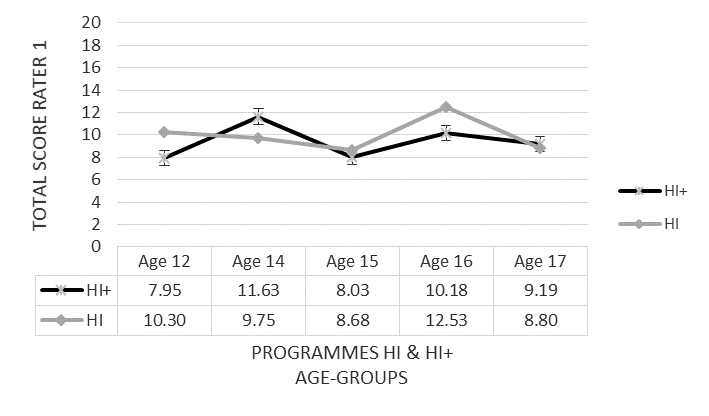
\includegraphics[width=4.7291in,height=2.7709in,width=\textwidth]{tejada-img2.png}

\end{center}
\begin{center}
 [Warning: Image ignored] % Unhandled or unsupported graphics:
%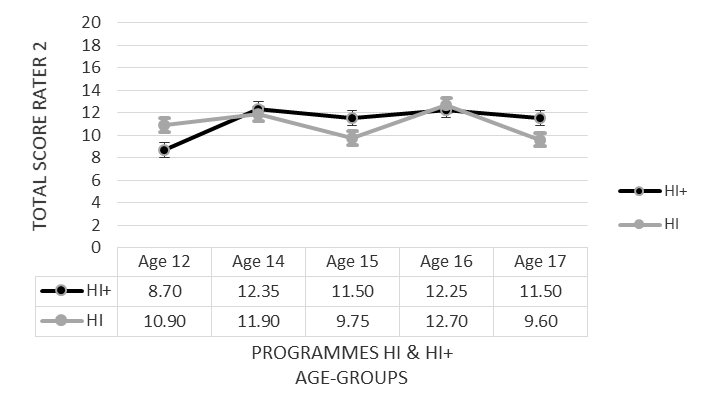
\includegraphics[width=4.7291in,height=2.7811in,width=\textwidth]{tejada-img3.png}

\end{center}
\begin{styleStandard}
Between-group comparisons using Welch’s t-test did not reveal any statistical differences between the programmes, as shown in Table 8. The mean difference between raters’ perception of HI+ and HI on various aspects of writing ability ranges from -0.17 to 0.03. These results suggest that neither programme is perceived as significantly different from the other, when it comes to the holistic rating of L2 writing performance. 
\end{styleStandard}

\begin{flushleft}
\tablehead{}
\begin{supertabular}{m{0.95315987in}m{0.49695984in}m{0.49275985in}m{0.7587598in}m{0.7268598in}m{0.5476598in}m{0.62755984in}m{0.47055987in}}
 &
\bfseries Group HI+\newline
Mean\newline
(SD) &
\bfseries Group HI\newline
Mean\newline
(SD) &
{\bfseries Mean Difference}

\bfseries Between groups &
\bfseries \textit{t} &
\bfseries \textit{p} &
\bfseries 95\% CI &
\bfseries \textit{d}\\\hline
\bfseries Task\newline
Fulfillment &
\mdseries 2.895\newline
(0.69) &
\mdseries 2.928\newline
(0.93) &
{\mdseries {}-0.033}

 &
\mdseries 0.191 &
\mdseries 0.84 &
\mdseries {}-0.293 0.355 &
{\mdseries 0.03}

\\\hline
\bfseries Text \newline
Organisation &
\mdseries 2.355\newline
(0.51) &
\mdseries 2.525\newline
(0.82) &
{\mdseries {}-0.170}

 &
\mdseries 1.15 &
\mdseries 0.253 &
{\mdseries {}-0.112 \ 0.422}

 &
{\mdseries 0.23}

\\\hline
{\bfseries \newline
Grammar}

 &
{\mdseries \newline
2.615 \newline
(0.60)}

 &
{\mdseries \newline
2.628 \newline
(0.74)}

 &
{\mdseries {}-0.012}

 &
{\mdseries 0.008}

 &
{\mdseries 0.992}

 &
{\mdseries {}-0.264 \ 0.266}

 &
{\mdseries 0.001}

\\\hline
\bfseries Vocabulary &
{\mdseries 2.53\newline
(0.64)}

 &
{\mdseries 2.50 \newline
(0.74)}

 &
{\mdseries 0.030}

 &
{\mdseries {}-0.334}

 &
{\mdseries 0.738}

 &
\mdseries {}-0.317 \ 0.225 &
\mdseries {}-0.06\\\hline
\bfseries TotalScore &
\mdseries 10.395\newline
(2.17) &
\mdseries 10.520 \newline
(2.97) &
{\mdseries {}-0.125}

 &
\mdseries 0.161 &
{\mdseries 0.871}

 &
{\mdseries {}-0.939 1.106}

 &
{\mdseries 0.03}

\\\hline
\end{supertabular}
\end{flushleft}
\begin{styleStandard}
\textit{Table 8: Analysis of between-group differences in holistic ratings by two evaluators (Welch’s T-Test)} 
\end{styleStandard}


\begin{listWWNumxxiileveli}
\item 
\begin{stylelsSectioni}
Discussion and conclusions
\end{stylelsSectioni}

\end{listWWNumxxiileveli}
\begin{styleStandard}
This study has sought to understand whether the differential accumulated time of EFL-exposure (expressed in number of hours of L2 learning) has an impact on writing performance in two immersion programmes, \ HI+ and \ HI. They are different in the accumulated number of hours at all points throughout the programme, and clearly at the end, at learners’ 17 years of age, when the HI+ programme has accumulated 8,760 \ hours, while the HI programme 7,002. 
\end{styleStandard}

\begin{styleStandard}
CAF measures and holistic ratings of writing samples were scrutinised with a cross-sectional design in which learners were measured throughout the programme, on a yearly basis, starting at age 12. Concerning CAF, four measures out of nine (IndepCS, CoordCR, DepCS, Guiraud, D, TotalErr/100, GrErr/100, WS, WM) were found to be statistically different between programmes but not all in favour of HI+. \ As regards complexity, IndepCS and DepCS \ were significantly lower for the HI+ group; \ for accuracy, GrErr/100 were statistically higher for the HI+ group; \ for fluency, WS, again, was statistically lower for the HI+ group. In terms of lexical complexity and the holistic ratings, no significant differences were found between the two programmes. 
\end{styleStandard}

\begin{styleStandard}
Overall, it would seem to be the case that the two programmes are not substantially different in terms of learners’ outcomes in EFL written performance. However, it cannot be said that they are entirely the same either. Indeed, the HI+ programme reveals lower levels in the domains of syntactic complexity and fluency, but higher levels for accuracy, and equal levels for lexical complexity. \ This has been also found in studies on the effects of a CLIL course in English added to conventional formal instruction contrasted with a group only taking formal instruction, as the latter outperformed the former, although not significantly (Pérez-Vidal \& Roquet 2015). 
\end{styleStandard}

\begin{styleStandard}
Consequently, given its mixed results, this study partly questions the early assertions made by Carroll (1962) and Stern (1985) in the direction that more L2-exposure time would directly lead to more skilled language use. Our approach to the interpretation of these findings is in terms of time distribution of each of the two programmes, between learners’ ages 12 and 17, as presented in Table 2 and Figure 1. In the case of HI+, learners undergo a decrease of L2-exposure time which goes from 672 hours a year to 612, and then to 480 (see Figure 1). This is not the case for HI pupils, who \ receive fewer hours of target language exposure per year, 504, yet at a steady rhythm. Additionally, the reduction in exposure is placed one year earlier for the HI+ group, that is at age 15, \ than for the HI group, at age 16.
\end{styleStandard}

\begin{styleStandard}
\ On the one hand, such a contrast in the distribution of L2 exposure time in the two programmes allows us to suggest that gradual exposure to the L2 (HI programme) might explain the similarity in results with HI+, with more accumulated amount of L2 exposure yet less consistent in its distribution.
\end{styleStandard}

\begin{styleStandard}
However, such a constant exposure experienced by the HI learners may also have had a less positive consequence; that is, the HI learners’ relative lower scores in terms of grammatical accuracy. In this sense, the notion of \textit{stabilisation}, or\textit{ plateauing}, proposed by Long (2003) might be relevant. Indeed, a closer analysis of the learners’ performance suggests a plateau effect mainly concerning grammatical accuracy, in the case of the HI programme predominantly observed in conjugation and agreement errors, a finding which has already been identified in immersion learners in the literature (Rifkin 2005, Hart, Lapkin \& Swain 1991). HI’s outcomes in accuracy could be interpreted as a level of {\textquotedbl}maintenance{\textquotedbl} achieved in this programme. These findings can be relative to the regular and steady amount of exposure for HI students in primary and between ages 12 and 15 in secondary school, as exposed in Figure 1.
\end{styleStandard}

\begin{styleStandard}
On this note, Bournot-Trites’ (2007) findings are only partially confirmed in our case. In her study, no significant differences in writing quality were found between two groups of secondary immersion students with different L2-French intensity. In addition, Bournot-Trites’ study reveals a plateau effect in the field of grammar accuracy (particularly tense markers) and lexical diversity, where she observes: {\textquotedbl}it seems that after a certain threshold of competence in [L2], the increase in the time spent in this language in the class does not improve much the quality of the written production of pupils{\textquotedbl} (p.20). \ 
\end{styleStandard}

\begin{styleStandard}
Likewise, the similarity of the two programmes in terms of lexical complexity could also be explained in terms of input exposure. It would seem that neither programme offers complementary hours of exposure outside of the classroom which would aid learners to make progress in such a domain. 
\end{styleStandard}

\begin{styleStandard}
Concerning the lower levels of fluency found in the HI+ group, they could be attributed either to the programme’s didactic approach, or to task effects which remain to be explored in future research. \ 
\end{styleStandard}

\begin{styleStandard}
Some limitations of this study need to be acknowledged. First the unbalance in the sample size where the HI+ programme includes a larger number of subjects than HI, which is represented by fewer subjects. Second, task conditions as well as task variety (in terms of complexity and text genres) need to be reconsidered. Further research might include different types of tasks and writing genres with different cognitive demands. We should additionally underscore that the HI programme-related positive results, which refer to denser, richer texts, may be associated to the emphasis on literacy in the HI’s curriculum described in section 4.1.1. The task might have been more familiar to HI students and therefore yielded to slightly more syntactically complex and organised texts. 
\end{styleStandard}

\begin{styleStandard}
To conclude, the present study has confirmed that the examination of the time factor in L2-acquisition in formal educational settings remains a rather complex endeavour due to a number of methodological constraints and issues. It is difficult to assess different programmes at exactly the same times (in terms of age, L2 exposure, curriculum years), and to control for programme features. \ Future research is needed to pursue research in bilingual schools or immersion programmes in non-English speaking contexts and to explore performance differences among different age groups, with a mixed methods approach including the holistic analyses suggested.
\end{styleStandard}

\begin{stylelsSectioni}
Acknowledgments
\end{stylelsSectioni}


\begin{styleStandard}
The authors are grateful to the anonymous reviewer as well as to Gabriele Pallotti for their insightful comments and contributions to this chapter. Also we would like to thank Cylcia Bolibaugh for her statistical advice. Isabel would like to thank Alejandra Plata and Alejandro Mejia from Uniandes for their help with earlier versions of this text.
\end{styleStandard}

\begin{stylelsSectioni}
References
\end{stylelsSectioni}


\begin{styleStandard}
Bardovi-Harlig, Kathleen. 1992. A Second Look at T-Unit Analysis: Reconsidering the Sentenc\textit{e. TESOL Quarte}rly 26(2). 390–395.
\end{styleStandard}


\begin{styleStandard}
Bournot-Trites, Monique. 2007. Qualité de l’écrit au niveau intermédiaire en immersion française[202F?]: effet d’un programme intensif et hypothèse d’un effet de plateau. \textit{Canadian Journal of Applied Linguistics / Revue canadienne de linguistique appliquée} 10(1). 7-23.
\end{styleStandard}


\begin{styleStandard}
Bonilla Carvajal, Camilo Andrés \& Isabel Tejada-Sánchez. 2016. Unanswered questions in Colombia’s language education policy. \textit{PROFILE Issues in Teachers’ Professional Development} 18(1). 185-201. 
\end{styleStandard}


\begin{styleStandard}
Bulté, Bram \& Alex Housen. 2014. Conceptualizing and measuring short-term changes in L2 writing complexity. \textit{Journal of Second Language Writing }26. 42–65.
\end{styleStandard}


\begin{styleStandard}
Bulté, Bram \& Alex Housen. 2012. Defining and Operationalising L2 complexity. In A. Housen, F. Kuiken \& I. Vedder (eds.), \textit{Dimensions of L2 Performance and Proficiency: Complexity,}\textit{ Accuracy and Fluency in SLA}, 21–46. Amsterdam/Philadelphia: Benjamins.
\end{styleStandard}


\begin{styleStandard}
Carroll, John Bissell. 1962. \textit{The Prediction of Success in Intensive Foreign Language Training} (Reprint from Training Research and Education), 87-136. Pittsburgh: University of Pittsburgh Press.
\end{styleStandard}


\begin{styleStandard}
Collins, Laura, Randall H. Halter, Patsy M. Lightbown \& Nina Spada. 1999. Time and the Distribution of Time in L2 Instruction. \textit{TESOL Quarterly} 33(4). 655. 
\end{styleStandard}


\begin{styleStandard}
Collins, Laura \& Joanna White. 2011. An Intensive Look at Intensity and Language Learning. \textit{TESOL Quarterly: A Journal for Teachers of English to Speakers of Other Languages and of Standard English as a Second Dialect} 45(1). 106–133. 
\end{styleStandard}


\begin{styleStandard}
Council of Europe. 2001. \textit{Common European framework of reference for languages: learning, teaching, assessment}. Cambridge: Press Syndicate of the University of Cambridge.
\end{styleStandard}


\begin{styleStandard}
Crystal, David. 1982. Profiling Linguistic Disability. London: Edward Arnold. 
\end{styleStandard}


\begin{styleStandard}
Dalton-Puffer, Christiane, Tarja Nikula, \& Ute Smit (eds.). 2010. \textit{Language Use and Language Learning in CLIL Classrooms. }Amsterdam: John Benjamins.
\end{styleStandard}


\begin{styleStandard}
Day, Elaine M. \& Stan Shapson. 1988. A Comparison Study of Early and Late French Immersion Programs in British Columbia. \textit{Canadian Journal of Education / Revue canadienne de l’éducation} 13(2). 290–305. 
\end{styleStandard}


\begin{styleStandard}
De Mejia, Anne-Marie. 2002. \textit{Power, Prestige and Bilingualism: International Perspectives on Elite Bilingual Education }(Bilingual Education and Bilingualism), 344. Clevedon: Multilingual Matters.
\end{styleStandard}


\begin{styleStandard}
Del Rio e.a.
\end{styleStandard}


\begin{styleStandard}
Ellis, Rod \& Gary Barkhuizen. 2005. \textit{Analysing Learner Language}, 404. Oxford: Oxford University Press.
\end{styleStandard}


\begin{styleStandard}
Friedl, Gabriele \& Margit Auer. 2007. “Assessment Scale for Writing.” Erläuterungen zur Novellierung der Reifeprufungsverordnung fur AHS, lebende Fremdsprachen. Novelle der Reifeprufungsverordnung gütlig ab dem Sommertermin 2009. 98. Wien/St. Pölten. Retrieved from: \url{http://docplayer.org/11483802-Novelle-der-reifepruefungsverordnung-2007-gueltig-ab-dem-sommertermin-2009-unter-beruecksichtigung-der-rpvo-novelle-2008.html} 
\end{styleStandard}


\begin{styleStandard}
Gensesee, Fred \& M.H. Stanley. 1976. The Development of English Writing Skills in French immersion School Programs. \textit{Canadian Journal of Education/ Revue canadienne de l’éducation} 1(3). 1-17.
\end{styleStandard}


\begin{styleStandard}
Genesee, Fred. 1978. Scholastic effects of French immersion: An overview after ten years. \textit{Interchange} 9(4). 20–29. 
\end{styleStandard}


\begin{styleStandard}
Genesee, Fred. 2013. Insights into Bilingual Education from Research on Immersion Programmes in Canada. In C. Abello-Contesse, P. M. Chandler, M. D. López-Jiménez \& R. Chacón-Beltrán (eds.), \textit{Bilingual and Multilingual Education in the 21st Century: Building on Experience (Bilingual Education and Bilingualism)}, \ 24–41. Bristol: Multilingual Matters. 
\end{styleStandard}


\begin{styleStandard}
Germain, Claude, Joan Netten \& Serge Séguin. 2004. L{\textquotesingle}évaluation de la production écrite en français intensif: Critères et resultats. \textit{The Canadian Modern Language Review }60(3). 333-353.
\end{styleStandard}


\begin{styleStandard}
Greenbaum, Sidney \& Randolph Quirk. 1990. \textit{A Student’s Grammar of the English Language}, 490. Harlow: Longman. 
\end{styleStandard}


\begin{styleStandard}
Grosjean, François. 2010. \textit{Bilingual: Life and Reality}, 304. Cambridge: Harvard University Press.
\end{styleStandard}


\begin{styleStandard}
Gunnarsson, Cecilia. 2012. \ The development of complexity, accuracy and fluency in the written production of L2 French. In A. Housen, F. Kuiken \& I. Vedder (eds.), \textit{Dimensions of L2 Performance and Proficiency: Complexity,}\textit{ Accuracy and Fluency in SLA}, 247 – 276. Amsterdam/Philadelphia: Benjamins.
\end{styleStandard}


\begin{styleStandard}
Harklau, Linda. 2002. The role of writing in classroom second language acquisition. \textit{Journal of Second Language Writing} 11(4). 329–350. 
\end{styleStandard}


\begin{styleStandard}
Harley, Birgit. 1992. Patterns of second language development in French immersion. \textit{French Language Studies} 2(2). 159–183.
\end{styleStandard}


\begin{styleStandard}
Hart, Doug, Sharon Lapkin \& Merrill Swain. 1991. Secondary Level Immersion French Skills: A Possible Plateau Effect. In L. Malavé \& G. Duquette (eds.), \textit{Language, Culture and Cognition: A Collection of Studies in First and Second Language Acquisition}, 250–265. Clevedon: Multilingual Matters.
\end{styleStandard}


\begin{styleStandard}
Housen, Alex \& Folkert Kuiken (2009). Special issue: Complexity, accuracy, fluency (CAF) in second language acquisition. \textit{Applied Linguistics} 30(4).
\end{styleStandard}


\begin{styleStandard}
Housen, Alex. 2012. Time and amount of L2 contact Inside and Outside the School - Insights from European Schools. In C. Muñoz (ed.), \textit{Intensive exposure experiences in second language learning}, 111–138. Bristol: Multilingual Matters.
\end{styleStandard}


\begin{styleStandard}
Housen, Alex, Folkert Kuiken \& Ineke Vedder. 2012. Complexity, accuracy and fluency. Definitions, measurement and research. In A. Housen, F. Kuiken \& I. Vedder (eds.), \textit{Dimensions of L2 Performance and Proficiency: Complexity,}\textit{ Accuracy and Fluency in SLA}, 1–20. Amsterdam/Philadelphia: Benjamins.
\end{styleStandard}


\begin{styleStandard}
Keaton, Buster. 1927. \textit{College}. Directed by James W. Horne \& Buster Keaton. Los Angeles: Joseph M. Schenck Productions.
\end{styleStandard}


\begin{styleStandard}
Hunt, Kellog W. 1965. A synopsis of clause-to-sentence length factors. \textit{The English Journal} 54(4). 300-309.
\end{styleStandard}


\begin{styleStandard}
Johnson, Robert Keith \& Merrill Swain. (1997). \textit{Immersion education[202F?]: international perspectives} (The Cambridge applied linguistics series), 315. Cambridge: Cambridge University Press.
\end{styleStandard}


\begin{styleStandard}
Juan-Garau, Maria \& Joana Salazar-Noguera. 2015. \textit{Content-based Language Learning in Multilingual Educational Environments}. Berlin: Springer. 
\end{styleStandard}


\begin{styleStandard}
Lambert, Monique. 1997. En route vers le bilinguisme. \textit{Acquisition et interaction en langue étrangère} 9. Online: \url{http://aile.revues.org/732} 
\end{styleStandard}


\begin{styleStandard}
Lambert, Wallace E. \& Richard G. Tucker. 1972. \textit{The bilingual education of children. The St. Lambert experiment.} Rowley: Newbury House Publishers.
\end{styleStandard}


\begin{styleStandard}
Larsen-Freeman, Diane. 1978. An ESL Index of Development. \textit{TESOL Quarterly} 12(4). 439–448.
\end{styleStandard}


\begin{styleStandard}
Lazaruk, Walter Andrew. 2007. Avantages linguistiques, scolaires et cognitifs de l’immersion française. \textit{Canadian Journal of Education / Revue canadienne de l’éducation} 63(5). 629–654.
\end{styleStandard}


\begin{styleStandard}
Lightbown, Patsy M. 2012. Intensive L2 Instruction in Canada: Why not Immersion?. In C. Muñoz (ed.), \textit{Intensive exposure experiences in second language learning}, 3–23. Bristol: Multilingual Matters.
\end{styleStandard}


\begin{styleStandard}
Long, Michael H. 2003. Stabilization and Fossilization in Interlanguage Development. In[202F?]C.J. Doughty \& M. H. Long (eds.), \textit{The Handbook of Second Language Acquisition, }487-535. Oxford: Blackwell Publishing Ltd. 
\end{styleStandard}


\begin{styleStandard}
MacWhinney, Brian. 2000. \textit{The CHILDES Project: Tools for Analyzing Talk.} Mahwah: Psychology Press.
\end{styleStandard}


\begin{styleStandard}
\textstyleStrong{\textmd{Malvern}}\textbf{, }David\textbf{ }D.,\textbf{~}\textstyleStrong{\textmd{Brian J. Richards}}\textbf{,~}\textstyleStrong{\textmd{Ngoni Chipere}}\textbf{ }\&\textbf{ }Pilar Duran. 2004. \textit{Lexical Diversity and Language Development} (Quantification and Assessment). New York: Palgrave Macmillan. 
\end{styleStandard}


\begin{styleStandard}
Malvern, David D. \& Brian J. Richards. 2000. Validation of a New Measure of Lexical Diversity. In M. Beers, B. v. d. Bogaerde, G. Bol, J. de Jong \& C. Rooijmans (eds.),\textit{ From Sound to Sentence: Studies on First Language Acquisition, }81-96\textit{. }Groningen: Centre for Language and Cognition.
\end{styleStandard}


\begin{styleStandard}
Manchón, Rosa M. 2009. \textit{Writing in Foreign Language Contexts: Learning, Teaching, and Research}. Bristol: Multilingual Matters. 
\end{styleStandard}


\begin{styleStandard}
Manchón, Rosa M. 2013. The Psycholinguistics of Bilingual Writing: Mapping the Terrain. In F. Grosjean \& P. Li (eds.), \textit{The Psycholinguistics of Bilingualism}, 102–116. Malden: Wiley-Blackwell.
\end{styleStandard}


\begin{styleStandard}
Meara, Paul \& Irma MIralpeix. 2017. Tools for researching vocabulary. Clevedon: Multilingual Matters.~
\end{styleStandard}


\begin{styleStandard}
Muñoz, Carmen. 2012. \textit{Intensive exposure experiences in second language learning}. \textit{Second language acquisition}, 258. Bristol: Multilingual Matters.
\end{styleStandard}


\begin{styleStandard}
Norris, John M. \& Lourdes Ortega. 2009. Towards an Organic Approach to Investigating CAF in Instructed SLA: The Case of Complexity. \textit{Applied Linguistics} 30(4). 555–578. 
\end{styleStandard}


\begin{styleStandard}
Ortega, Lourdes. 2003. Syntactic Complexity Measures and their Relationship to L2 Proficiency: A Research Synthesis of College level L2 Writing. \textit{Applied linguistics} 24(4). 492.
\end{styleStandard}


\begin{styleStandard}
Ortega, Lourdes. 2012. Epilogue: Exploring L2 Writing-SLA Interfaces. \textit{Journal of Second Language Writing} 21(4). 404–415. 
\end{styleStandard}


\begin{styleStandard}
Pallotti, Gabriele. 2015. A simple view of linguistic complexity. \textit{Second Language Research }31(1). 117-134. 
\end{styleStandard}


\begin{styleStandard}
Plonsky, Luke \& Frederick L. Oswald. 2014. How Big Is “Big”? Interpreting Effect Sizes in L2 Research. Methodological Review Article, \textit{Language Learning }64(4). 878–912. 
\end{styleStandard}


\begin{styleStandard}
Pérez-Vidal, Carmen. 2015. Perspectives and lessons from the challenge of CLIL experiences. In C. Abello-Contesse, P.M. Chandler, M.D. López-Jiménez \& R. Chacón-Beltrán (eds.), \textit{Bilingual and Multilingual Education in the 21}\textit{\textsuperscript{st}}\textit{ Century: Building on experience, }59-85\textit{. }Clevedon: Multilingual Matters. 
\end{styleStandard}


\begin{styleStandard}
Polio, Charlene. 1997. Measures of Linguistic Accuracy in Second Language Writing Research. \textit{Language Learning} 47(1). 101–143. 
\end{styleStandard}


\begin{styleStandard}
Polio, Charlene. 2001. Research methodology in second language writing: The case of text-based studies. In T. Silva \& P. Matsuda. (eds.), \textit{On second language writing}, 91-116. Mahwah, NJ: Erlbaum.
\end{styleStandard}


\begin{styleStandard}
Quirk, Randolph, Sidney Greenbaum, Geoffrey Leech \& Jan Svartvik. 1985. \textstyleHTMLCite{A Comprehensive Grammar of the English Language, }\textstyleHTMLCite{\textup{78}}. London: Longman.
\end{styleStandard}


\begin{styleStandard}
Read, John. 2000. \textit{Assessing Vocabulary}. Cambridge: Cambridge University Press.
\end{styleStandard}


\begin{styleStandard}
Rifkin, Benjamin. 2005. A Ceiling Effect in Traditional Classroom Foreign Language Instruction: Data from Russian. \textit{The Modern Language Journal} 89(1). 3–18. 
\end{styleStandard}


\begin{styleStandard}
Roquet, Helena \& Carmen Pérez-Vidal. 2015. The linguistic impact of a CLIL Science Programme: An analysis measuring relative gains. \textit{System} 54. 80-90. 
\end{styleStandard}


\begin{styleStandard}
Roquet, Helena \& Carmen Pérez-Vidal. 2015. Do productive skills improve in Content and Language Integrated Learning Contexts?: The case of writing. \textit{Applied Linguistics, 1-24. }
\end{styleStandard}


\begin{styleStandard}
Serrano, Raquel. 2007. \textit{Time Distribution and the Acquisition of English as a Foreign Language}. Barcelona: Universitat de Barcelona PhD Thesis.
\end{styleStandard}


\begin{styleStandard}
Serrano, Raquel, Àngel Llanes \& Elsa Tragant. 2011. Analyzing the effect of context of second language learning: Domestic intensive and semi-intensive courses vs. study abroad in Europe. \textit{System} 39(2). 133–143. 
\end{styleStandard}


\begin{styleStandard}
Serrano, Raquel \& Carmen Muñoz. 2007. Same hours, different time distribution: Any difference in EFL?. \textit{System} 35(3). 305–321. 
\end{styleStandard}


\begin{styleStandard}
Silva, Tony \& Paul Kei Matsuda (eds.). 2005. On Second Language Writing. Mahwah: Routledge.
\end{styleStandard}


\begin{styleStandard}
Skehan, Peter \& Pauline Foster. 1999. The Influence of Task Structure and Processing Conditions on Narrative Retellings\textit{. Language Learning} 49. 93–120. 
\end{styleStandard}


\begin{styleStandard}
Skehan, Peter. 2009. Modelling Second Language Performance: Integrating Complexity, Accuracy, Fluency, and Lexis. \textit{Applied Linguistics }30\textit{(4).}\textstyleappleconvertedspace{ }\textstyleslugpages{510-532.}
\end{styleStandard}


\begin{styleStandard}
\textstyleslugpages{Stern, Hans H. 1985. The time factor and the Compact Course Development. }\textit{TESL Canada }\textit{Journal/Revue Tesl du Canada }3(1). 13-29.
\end{styleStandard}


\begin{styleStandard}
Swain, Merrill. 1981. Time and timing in bilingual education. \textit{Language Learning} 31(1). 115.
\end{styleStandard}


\begin{styleStandard}
Swain, Merrill. 2000. French Immersion Research in Canada: Recent Contributions to SLA and Applied Linguistics. \textit{Annual Review of Applied Linguistics} 20. 199–212. 
\end{styleStandard}


\begin{styleStandard}
Tejada-Sanchez. Martha Isabel. 2014. L{\textquotesingle}acquisition de l{\textquotesingle}anglais et l{\textquotesingle}exposition intensive en contexte d{\textquotesingle}immersion scolaire en Colombie. Unpublished doctoral dissertation. Barcelona/Paris: Universitat Pompeu Fabra - Université Paris 8 PhD Thesis. 
\end{styleStandard}


\begin{styleStandard}
Torras, María Rosa, Teresa Navés, Maria Luz Celaya \& Carmen Pérez-Vidal. 2006. Age and IL development in writing. In C. Muñoz (ed.), \textit{Age and the Rate of Foreign Language Learning}, 156-182. Clevedon: Multilingual Matters.
\end{styleStandard}


\begin{styleStandard}
Turnbull, Miles, Sharon Lapkin, Doug Hart \& Merrill Swain. 1998. Time on task and immersion graduates’ French proficiency. In S. Lapkin (ed.), \textit{French second language education in Canada: Empirical studies}, 31–55. Toronto: University of Toronto Press.
\end{styleStandard}


\begin{styleStandard}
Vyatkina, Nina. 2012. The Development of Second Language Writing Complexity in Groups and Individuals: A Longitudinal Learner Corpus Study.\textit{ }\textit{The Modern Language Journal }96(4). 576-598.
\end{styleStandard}


\begin{styleStandard}
Weigle, Sara (Cushing). 2002. \textit{Assessing Writing}. 284. Cambridge: Cambridge University Press.
\end{styleStandard}


\begin{styleStandard}
Wesche, Marjorie Bingham. 1989. Les diplômés de l’immersion: implications dans le domaine de l{\textquotesingle}enseignement du français. \textit{The Canadian Journal of Higher Education }19(3). 30–41.
\end{styleStandard}


\begin{styleStandard}
Wesche, Marjorie Bingham. 2002. Early French Immersion: How Has the Original Canadian Model Stood the Test of Time. In P. Burmeister, T. Piske, \& A. Rohde (eds.), \textit{An Integrated View of Language Development. }\textit{Papers in Honor of Henning Wode, }23. Trier: WVT Wissenschaftlicher Verlag Trier.
\end{styleStandard}


\begin{styleStandard}
Williams, Jessica. 2012. The potential role(s) of writing in second language development. \textit{Journal of Second Language Writing} 21(4). 321–331. 
\end{styleStandard}


\begin{styleStandard}
Wolfe-Quintero, Kate, Shunji Inagaki \& Kim Hae-Young. 1998. \textit{Second Language Development in Writing: Measures of Fluency, Accuracy, and Complexity}, 208. Manoa: National Foreign Language Resource Center - University of Hawaii at Manoa.
\end{styleStandard}


\end{document}
